\fancyhf{}
\fancyhead[C]{Chapter 3. Neuromodulatory Control of Cortical Function:
Cell-Type Specific Reshaping of Neuronal
Information Transfer}% <- added
\fancyfoot[R]{\thepage\ifodd\value{page}\else\hfill\fi}
%\fancyhead[L]{\ifodd\value{page}\relax\else\hfill\fi Ch \thechapter}
%\renewcommand\headrulewidth{0pt}% default ist .4pt
\renewcommand{\plainheadrulewidth}{.4pt}% default is 0pt


\newpage
\section{Abstract}
\tab 
Neuromodulatory systems are crucial for cognitive flexibility, dynamically altering neuronal and circuit properties. However, how these systems control information transfer, particularly in a cell-type and receptor-specific manner, remains poorly understood. Here, we investigated how dopaminergic (D1-R, D2-R) and cholinergic (M1-R) receptor activation reconfigures the input-output processing of excitatory and inhibitory neurons in layer 2/3 of mouse somatosensory cortex. Using in-vitro whole-cell recordings under a Frozen Noise stimulus protocol, we characterized neurons by four sets of functional attributes: action potential dynamics, passive biophysical properties, adaptation currents, and input feature selectivity (via spike-triggered averages). We found that neuromodulator receptor activation alters information transfer between stimulus and spike train in a manner dependent on both cell type and receptor. Unsupervised clustering (UMAP+Louvain) of attribute sets revealed that neuromodulation dynamically reshapes neuronal functional identities. Critically, multi-set correlation and factor analysis (MCFA) demonstrated that neuromodulators reorganize the covariance structure between these attribute sets. For instance, D1-R and D2-R activation increased the independence of input feature selectivity (STA) in excitatory neurons while enhancing coordination among output-related features. Conversely, inhibitory neurons generally exhibited increased coordination across functional domains. These findings demonstrate that neuromodulators do not merely tune individual neuronal properties but orchestrate a complex, coordinated reconfiguration of the functional landscape, thereby dynamically reshaping the computational capabilities of cortical circuits.

\newpage
\section {Introduction}


Neuromodulators such as dopamine and acetylcholine play a critical role in shaping circuit development as well as brain states and cognitive functions, including attention, learning, memory, and sleep \cite{dalley2004cortical,hasselmo2006cholinergic,sarter2009phasic}. These molecules do not directly evoke neural activity but also modulate how neurons respond to synaptic input, tuning the input–output relationships of individual neurons. Disruptions in neuromodulatory systems have been implicated in neurological and psychiatric disorders such as Parkinson’s disease and schizophrenia \cite{durstewitz2008dual,arnsten2012neurobiological,winterer2004genes}.

Despite extensive work on their cellular and behavioral effects, it remains unclear how neuromodulators influence what neurons compute, specifically, how they encode and transmit information. Traditional approaches have primarily focused on measuring the effects of neuromodulation on single variable measures such as firing rate or spike-frequency adaptation \cite{nadim2014neuromodulation,marder2012neuromodulation,shine2021computational}. While informative, these scalar metrics fail to capture the complexity of neuronal computation, which emerges from the dynamic interaction of passive membrane properties, intrinsic excitability, synaptic integration, and stimulus selectivity. Furthermore, little is known about whether neuromodulatory effects act independently on each property or reshape the correlation between properties in a structured way, particularly in a receptor- and cell-type-specific manner.

Neurons are high-dimensional dynamical systems. Understanding how neuromodulation alters the relationships among functional attributes such as action potential dynamics, adaptation, and input filtering is critical for revealing how neurons adjust their computational roles within a circuit. Dopaminergic (via D1-R and D2-R) and cholinergic (via M1-R) signaling pathways are known to modulate ion channel activity and membrane excitability \cite{bargmann2012beyond, marder2012neuromodulation,taghert2012peptide}, thereby influencing both spike generation and input selection \cite{dascal2001ion,seong2012d1,cousineau2020dopamine}. These effects are mediated through receptors, expressions of which varies across cell types \cite{nusser2009variability}, suggesting that neuromodulators may reconfigure cortical circuits in a subtype-specific manner. Moreover, cell properties themselves are independent. For instance, passive properties such as membrane conductance shape downstream attributes like spike waveform and filtering dynamics \cite{hausser2000hodgkin,ferguson2020mechanisms,salinas2001book}, this raises the possibility that neuromodulatory effects may produce coordinated, rather than isolated, functional changes. To test this, we asked: How does receptor-specific neuromodulation reorganize the functional encoding landscape of cortical neurons?

We addressed this question using in-vitro whole-cell recordings from excitatory and inhibitory neurons in layer 2/3 of the mouse somatosensory cortex. Each neuron was stimulated with a biophysically realistic time-varying current generated by the Frozen Noise protocol (FN) \cite{zeldenrust2017estimating}, and recordings were obtained under control (aCSF) and receptor-specific agonist conditions (D1-R, D2-R, M1-R). This protocol allowed us to measure both the information transferred by each neuron and the detailed physiological attributes underlying that computation.

Firstly, we quantify how neuromodulation affects the amount of information that is transferred from the input of a neuron to its output \cite{zeldenrust2017estimating}. We find that neuromodulation changes information transfer in a cell-type specific manner. Secondly, we analyze the effects of neuromodulation in high-dimensional electrophysiological property space. From each recording, we extracted four sets of functional attributes: (1) action potential (AP) dynamics, (2) passive biophysical (PB) properties, (3) adaptation currents (AC), and (4) input filtering via spike-triggered average (STA). These feature sets each capture a different aspect of neuronal function, from passive to active (input-driven). We then examined whether receptor activation reorganized the functional identity of neurons. Specifically, for each set of attributes, we were interested to see whether neurons that would cluster together in unsupervised high-dimensional clustering (UMAP + Louvain) under the aCSF condition, would also cluster together under neuromodulation. Finally, we applied multi-set correlation and factor analysis (MCFA) to assess whether neuromodulation alters the correlation between attribute sets, reflecting a global reconfiguration of a neuronal population's computational architecture.

Together, these analyses reveal how dopaminergic and cholinergic modulation reshape the functional landscape of cortical neurons. By linking receptor-specific activation to changes in how neurons encode stimuli through shifts in high-dimensional functional attribute sets, this study provides a systems-level framework for understanding neuromodulation in both single neuron and circuit level which is crucial for studying disease such Parkinson's and schizophrenia as well development of biologically realistic neural networks.

 
%%%%%%%%%%%%%%%%%%%%%%%%%%%%%%%%%%%%%%%%%%%%%%%%%%%%%%%%%%%%%%%%%%%%%%%%
%%%%%%%%%%%%%%%%%%%%%%%%%%%%%% Methods    %%%%%%%%%%%%%%%%%%%%%%%%%%%%%%
%%%%%%%%%%%%%%%%%%%%%%%%%%%%%%%%%%%%%%%%%%%%%%%%%%%%%%%%%%%%%%%%%%%%%%%%

\section{Methods}







\textbf{Ethics statement} The data used in this research was previously published and made freely available to the community \cite{da2018databank} and \cite{yan2022whole}. All experimental work, as described in the articles cited, was carried out in accordance with the European directive 2010/63/EU, the Dutch national regulations and international standards for animal care and use.    

\begin{flushleft}
\textbf{Slice electrophysiology} The experimental procedures were described before \cite{da2018databank, yan2022whole}. In short, slices were prepared from adult mice expressing Cre recombinase under the control of either the parvalbumin promoter (RRID: MGI:5315557) or the somatostatin promoter (RRID: IMSR JAX:013044), backcrossed to the C57BL/6 background. The animals were housed in a 12-hour light / dark cycle with ad libitum access to food and water and kept in family cages until the day of the experiment.

The experimental procedures followed previously published protocols (\cite{Zeldenrust2018,Azarfar2018,Zeldenrust2017,Zeldenrust2017b,Celikel2004,Celikel2003}). Coronal slices (thickness: 300 microns) were cut from the barrel cortex subregion of the primary somatosensory cortex, and individual neurons were visualized using differential interference contrast (DIC) optics at 40× magnification before whole-cell access using pipettes with a resistance of 5-9 $M\Omega$. The internal (pipette) solution contained (in mM): 130 K-gluconate, 5 KCl, 1.5 $MgCl_2$·$6H_2O$, 0.4 $Na_3GTP$, 4 $Na_2ATP$, 10 HEPES, 10 Na-phosphocreatine, and 0.6 EGTA. The pH was adjusted to 7.22 with KOH. Recordings were performed using HEKA EPC10 amplifiers and PatchMaster software (v2x90.2). 

Targeted pharmacological activation of the select receptors was performed using agonists for the serotonin $5-HT_1F$ receptors (LY334370, 5$\cdot \mu M$), muscarinic acetylcholine M1 receptors (McN-A-343, 20$\cdot \mu M$), dopamine D1 (SKF38393, 1$\cdot \mu M$) and D2 receptors (Quinpirole, 10$\cdot \mu M$). All compounds were purchased from Sigma-Aldrich and dissolved in ACSF \cite{yan2022whole}.

Each neuron served as its own control, with baseline recordings acquired in ACSF prior to drug application. Drug effects were assessed beginning 3 minutes after compound introduction into the continuously perfused bath. Following each experiment, the recording chamber was thoroughly cleaned, and dedicated containers were used for each drug solution to prevent cross-contamination \cite{yan2022whole}.

\end{flushleft}



\begin{flushleft}
\textbf{Frozen Noise (FN) protocol} The Frozen Noise input protocol consisted of injecting a somatic current that is the result of an artificial neural network of 1000 neurons responding (firing Poisson spikes) to random stimuli i.e., the hidden state, the membrane potential response to the somatic input is recorded with a sampling rate of 20 kHz for a total length of 360 seconds and saved. Each raw data file consisted of a vehicle control trial (artificial Cerebrospinal fluid i.e. aCSf)  and a drug trial (a specific neuromodulatory receptor agonist or antagonist was added to the bath and the recording was repeated). Some files consisted of multiple control and drug trials. See \cite{zeldenrust2017estimating,da2018databank} for more details. A schema for the protocol is shown in Fig. \ref{fig:FN_protocol}. In total 288 neurons (Table. \ref{tab:neuron_table}) were analyzed, we discarded recording sets with high levels of noise.   

\begin{table}[!htb]
    \centering
    \begin{tabular}{c|c|c}
 \hline
 Condition & Cell-type &Trials\\
 \hline
         aCSF & Excitatory & 183\\
         aCSF & Inhibitory & 121 \\       
         D1   & Excitatory & 50\\
         D1   & Inhibitory & 36\\         
         D2   & Excitatory & 40\\
         D2   & Inhibitory & 19\\
         M1   & Excitatory & 19\\
         M1   & Inhibitory & 20\\

\hline         
    \end{tabular}
    \caption{Number of recording set for control and agonist conditions}
    \label{tab:neuron_table}
\end{table}

\end{flushleft}

%%%  Please list here under separate headings 
%%%  all the experimental models/study participants 
%%%  (animals, human participants, plants, microbe 
%%%  strains, cell lines, primary cell cultures) 
%%%  used in the study. For each model, provide 
%%%  information related to their species/strain, 
%%%  genotype, age/developmental stage, sex (and 
%%%  gender, ancestry, race, and ethnicity if 
%%%  reported for human studies), maintenance, 
%%%  and care, including institutional permission 
%%%  and oversight information for the studies 
%%%  the experimental animal/human participant 
%%%  study. The influence (or association) of sex, 
%%%  gender, or both on the results of the study 
%%%  must be reported. In cases where it cannot, 
%%%  authors should discuss this as a limitation 
%%%  to their research’s generalizability.

%%%  Please omit this component if your study does 
%%%  not use experimental models typical in the 
%%%  life sciences (e.g., if your study is 
%%%  computational or physical science research). 

\subsection*{Analysis}

\subsubsection*{Feature Extraction} 
\begin{flushleft}
We extracted waveform, action potential, passive biophysical and spike triggered average from single neuron recordings recorded under Frozen Noise input protocol, these recordings were performed first under a vehicle control (aCSF) and then repeated with a receptor agonist added to the bath. 
\end{flushleft}

\begin{flushleft}
\textbf{Spike waveforms} As explained in \cite{joshi2024understanding}, we identified peaks from the membrane potential traces and kept the hyperparameters and ISI threshold criteria the same as in \cite{joshi2024understanding}. The length of the waveforms used in this study is 10ms (5ms before and after the peak).      
\end{flushleft}

\begin{flushleft}
\textbf{Action potential attributes} 
The action potential attributes were extracted to study the dynamics, threshold and waveforms related attributes throughout a trial via descriptive statistics.  The action potential attributes were extracted for aCSF and agonist trails as described in \cite{joshi2024understanding}. A summary of all the Action potential attributs is provided in Table. \ref{tab:ap_features}. 
\end{flushleft}

\begin{table}[H]
\centering

\begin{tabular}{p{2.2cm}|p{2cm}|p{4cm}|p{3.5cm}}
\hline
\textbf{Feature Group}  & \textbf{Feature} & \textbf{Description}& \textbf{Summary Statistics}\\
\hline

{Spiking Dynamics}& Current at first spike & Current amplitude at which the neuron first crosses threshold to fire a spike. &Single value per trial.\\
% \cline{2-3}
 & AP count & Total number of action potentials generated during a trial. &Single value per trial.\\
% \cline{2-3}
 & Time to first spike & Time (in ms) from trial start to first spike. &Single value per trial.\\
% \cline{2-3}
 & Firing rate & Total number of spikes divided by trial duration (spikes/sec).& Single value per trial.\\
% \cline{2-3}
 & Interspike Interval (ISI) & Time between successive spikes ($t_{n+1} - t_n$). &Mean, median, max, min calculated.\\
 & Instantaneous rate & Reciprocal of ISI ($1 / (t_{n+1} - t_n)$). &Mean, median, max, min calculated.\\
\cline{1-3}

{Spike Threshold}& Spike threshold & Voltage at which $dV/dt$ first exceeds 25 mV/ms. Calculated per spike. & Mean, median, 
max, min computed.\\
\cline{1-3}

{AP Height \& Width}& Width & Time from threshold crossing to return below threshold after AP peak. &Mean, median, max, min calculated.\\
 & Amplitude & Voltage difference between AP peak and threshold. & Mean, median, max, min calculated.\\ 
\hline
\end{tabular}
\caption{Summary of Action Potential Attributes and Their Descriptions}
\label{tab:ap_features}
\end{table}

% \newpage
\subsubsection*{Passive Biophysical Feature extraction using GLIF model}
In order to extract passive biophysical attributes as well as adaptation current from aCSF and agonist trials, we fit a Generalized Leaky Integrate and Fire (GLIF) neuron model  \cite{pozzorini2015automated} as described in detail in \cite{joshi2024understanding}. We take the first 100 second from the recording as the training set to extract passive attributes as well as adaptation current from the recording. A summary of all the passive biophysical features extracted is provded in Table. \ref{tab:passive_biophys_features}.  Using the same GLIF model fitted to neural recordings, we also extracted the adaptation current $\eta(t)$ triggered by a spike event, see \cite{joshi2024understanding,pozzorini2015automated}. 


\begin{table}[H]
\centering
\begin{tabular}{p{4cm}|p{8cm}}
\hline
\textbf{Feature} & \textbf{Description} \\ \hline
Membrane Capacitance ($C$) & The cell membrane’s ability to store charge; influences how quickly voltage changes in response to current. \\ \hline
Leak Conductance ($g_L$) & Governs the passive flow of ions across the membrane; contributes to the rate of membrane potential decay. \\ \hline
Resting Potential ($E_L$) & The membrane voltage the cell settles at in the absence of input; baseline membrane potential. \\ \hline
Sharpness of Spike Threshold ($\Delta V$) & Controls how sharply the firing probability increases as membrane potential approaches threshold. \\ \hline
Threshold Baseline ($V_T^*$) & The baseline value of the dynamic spike threshold; determines the average voltage required to trigger a spike. \\ \hline
Reset Voltage ($V_{reset}$) & The membrane potential value the neuron resets to after a spike and refractory period. \\ \hline
\end{tabular}
\caption{Passive Biophysical Features Extracted from the GLIF Model}
\label{tab:passive_biophys_features}
\end{table}

\paragraph{Spike Triggered Average} The spike-triggered average (STA) is the average shape of the stimulus that precedes each spike. We extracted the STA using the following equation given by \cite{schwartz2006spike}: 
\begin{equation}
STA = \frac{1}{N}\Sigma_{n=1}^{N}  \overrightarrow{s}(t_{n}),    
\end{equation}
\begin{flushleft}
where $t_n$ is the $n^{th}$ spike time, s is the stimulus vector preceding the spike for a fixed time window of 100 ms, and N is the total number of spikes. Before clustering, we standardize (i.e. z score) and then normalize the STA vector with an $L_2$ norm. We didn't use any kind of whitening or regularization to calculate the STA.      
\end{flushleft}



% \subsubsection{\textbf{CLUSTERING METHOD}}
\subsection*{UMAP + Louvain clustering} 
\label{sec:clustering_meth}
Universal Manifold Approximator (UMAP) is a non-linear dimensionality reduction algorithm which is advantageous for preserving global structure of the data \cite{mcinnes2018umap} in lower dimensions, this makes it more suitable for visualization especially for high dimensional datasets ($p>>N$, where p is the dimensionality of the data and N is number of samples) compared to other methods such as PCA which fail to perform due to curse of dimensionality \cite{aggarwal2001surprising}.  As explained in \cite{lee2021non,joshi2024understanding} the high-dimensional graph obtained during the intermediate step in the UMAP algorithm can be exploited to perform clustering using Louvain community detection \cite{blondel2008fast}. We chose the hyperparameter based on cluster stability criteria and the corresponding number of clusters based on the same heuristic as explained in \cite{joshi2024understanding}.  

For measuring clustering similarity between aCSF and drug conditions, we calculate a cluster similarity matrix as explained in \cite{joshi2024understanding}. For quantifying the similarity between labels assigned to aCSF versus drug trials, we used cluster similarity measure such as adjusted random index and adjusted mutual information score using scikit-learn Python package \cite{scikit-learn}.     

\subsection{Information transfer protocol}
We employed the information transfer protocol detailed in \cite{zeldenrust2017estimating, zeldenrust2024tuning} to quantify how much information a single neuron extracts from its inputs. This protocol assumes that neurons respond to the presence or absence of a preferred stimulus, which is modeled as a binary hidden state ($\mathbf{x}$) that switches between 0 and 1 according to a memoryless Markov process. Importantly, the neuron does not directly observe this hidden state; instead, it receives input from a large population of simulated presynaptic neurons. Each presynaptic neuron fires a Poisson spike train, with firing rates $q_{on}^i$ when the hidden state is ON ($x=1$), and $q_{off}^i$ when it is OFF ($x=0$).

To generate the input current ($\mathbf{I}$), the spike train of each presynaptic neuron is convolved with a 5~ms exponential kernel and then weighted by $w_i = \log\left(\frac{q_{on}^i}{q_{off}^i}\right)$. The weighted signals are summed to produce the total input current, which is then scaled and injected as somatic input during in vitro patch-clamp recordings. The neuron's membrane potential and spike times are recorded in response to this current (Fig. \ref{fig:FN_protocol}).

Information transfer is quantified in several steps. First, the entropy of the hidden state ($H_{xx}$) is calculated. Next, the mutual information between the hidden state and the input current ($MI_I$), and between the hidden state and the neuron's spike times ($MI_{\text{spike times}}$), are computed. The fraction of information (FI) transferred by the neuron is then defined as:
\begin{equation}
    FI = \frac{MI_{\text{spike times}}}{MI_I}
\end{equation}

Since the entropy of the hidden state is always greater than or equal to the mutual information, $FI$ values range between 0 and 1. This approach assumes ergodicity (so time averages equal ensemble averages) and that spike trains are approximately Poissonian, though minor deviations from Poisson statistics do not significantly affect the results. By using a binary hidden state, this protocol allows for reliable estimation of mutual information even from relatively short recordings, providing a robust measure of how effectively a neuron's spikes encode information about dynamic stimuli.

\begin{figure}
    \centering
    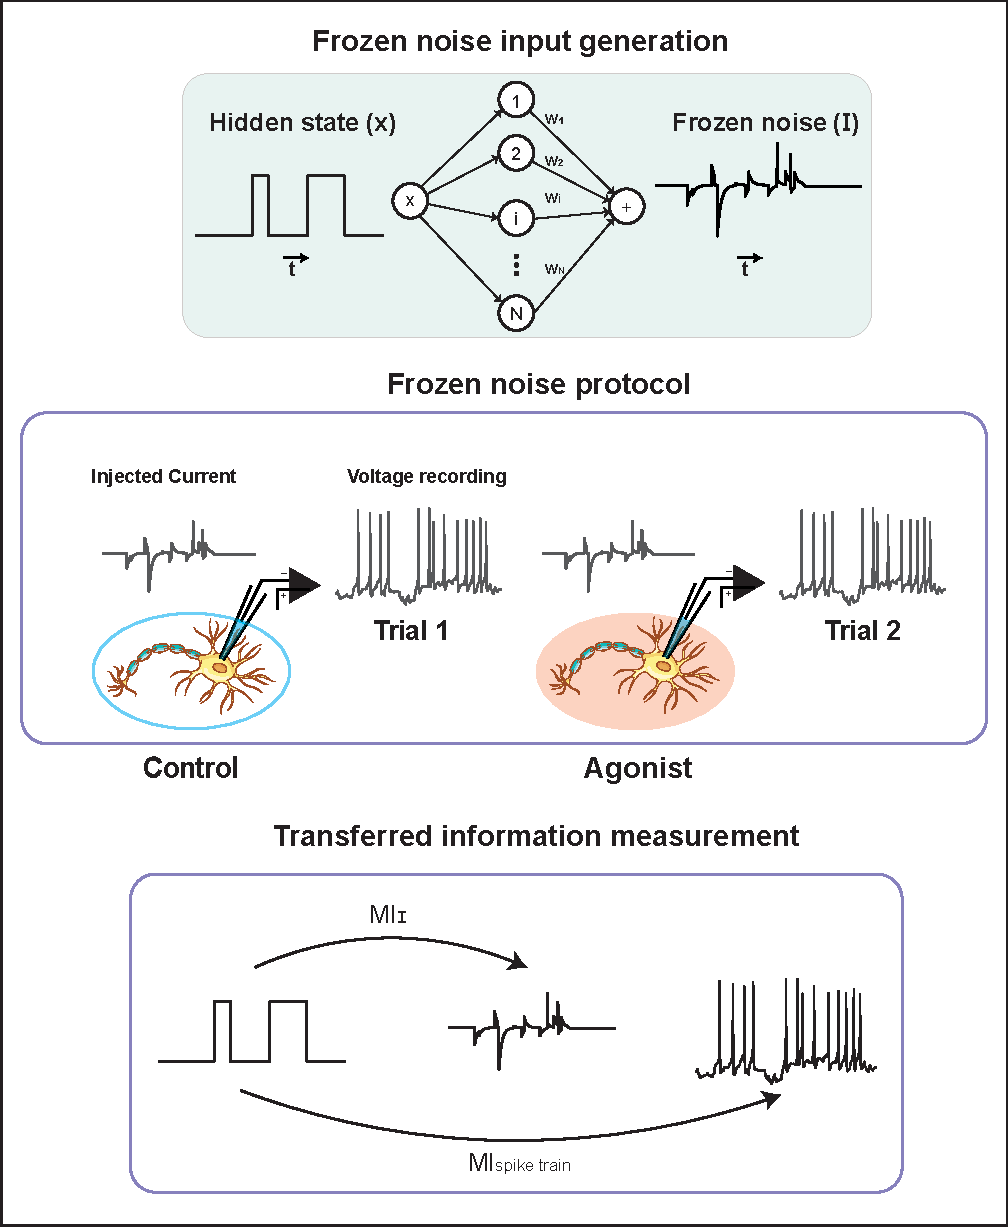
\includegraphics[width=
    \linewidth]{Figures/Ch_3/Fig1.pdf}
    \caption{\textbf{Frozen noise protocol}: The top figure provides an illustration of how input is generated, the middle figure illustrates how this input is injected into the soma of a neuron for both aCSF and agonist conditions, the bottom figure illustrates the schema for calculating mutual information. }
    \label{fig:FN_protocol}
\end{figure}
\subsection*{Quantification and statistical analysis}
We used the non-parametric Wilcoxon test to test the significance of the observed difference in information transfer (FI) between paired aCSF and drug trials . We also used one sided Student's T-test to test the significance of the observed change between aCSF and agonist condition for passive biophysical and action potential attributes. Significance value was set to $p<0.05$ in both cases.  We performed a Kruskal-Wallis H test and a post-hoc Mann-Whitney U test with Bonferroni correction for multiple comparisons for comparing the cosine similarity between aCSF and agonist trials. All statistical tests were performed using scipy-stats package \cite{2020SciPy-NMeth}.  
 

\subsection*{Multi-set Correlation and Factor Analysis}

To investigate how neuromodulation alters the relationship between different functional attribute sets (AP, PB, AC, and STA), we used \textbf{Multi-set Correlation and Factor Analysis (MCFA)} \cite{brown2023multiset}, an unsupervised integration method designed to model both shared and private variance across multiple high-dimensional data types from the same samples. This method combines elements of canonical correlation analysis and factor analysis to produce low-dimensional representations of common and dataset-specific structure.

Each attribute set was z-scored (mean-centered and variance-scaled), and MCFA was applied separately to aCSF and agonist conditions. For the aCSF condition, we fixed the number of principal components to 2 for all attribute sets, due to the relatively low dimensionality of AP and PB features (e.g., PB: 6 dimensions). Private latent dimensionality $k_m$ was also set to 1 for each set, based on model stability and convergence tests. Attempts to use higher latent dimensions resulted in non-convergent fits. These same dimensionality parameters (PCs = 2, $k_m$ = 1 ) were applied to agonist conditions to maintain consistency and due to smaller sample sizes in drug trials.

Since the number of aCSF recordings exceeded the number of agonist trials, we bootstrapped the control condition by randomly sampling subsets matched in size to the agonist group with the least number of recording sets, i.e., M1-R. This process was repeated 100 times, and MCFA was run on each subset. The resulting shared and private variances were averaged across runs to produce stable estimates for the control condition.

The MCFA fitting procedure used an expectation-maximization (EM) algorithm as described in \cite{brown2023multiset}, initialized according to \cite{joshi2024understanding}. Convergence was assessed by monitoring the log-likelihood and change in loading matrices across iterations.




%%%%%%%%%%%%%%%%%%%%%%%%%%%%%%%%%%%%%%%%%%%%%%%%%%%%%%%%%%%%%%%%%%%%%%%%
%%%%%%%%%%%%%%%%%%%%%%%%%%%%%% Results    %%%%%%%%%%%%%%%%%%%%%%%%%%%%%%
%%%%%%%%%%%%%%%%%%%%%%%%%%%%%%%%%%%%%%%%%%%%%%%%%%%%%%%%%%%%%%%%%%%%%%%%

\section{Results}



Neuronal identity is shaped by both intrinsic properties, such as gene expression and ion channel makeup \cite{schultz2007multiple,fishell2013neuron}, and external influences like synaptic input \cite{joshi2024understanding} and neuromodulatory signals. While previous work has studied excitability effects, it is still unclear how specific neuromodulators reconfigure a neuron’s functional role across different physiological domains. 

This study investigates how selectively activating dopaminergic (D1-R, D2-R) and cholinergic (M1-R) receptors modifies the input–output properties of excitatory and inhibitory neurons. We used the single unit somatic in-vitro recording dataset (\cite{yan2022whole}), in which the neurons were recorded using the Frozen Noise (FN) protocol \cite{zeldenrust2017estimating} (see Methods and Fig. \textbf{\ref{fig:FN_protocol}}) to capture responses under biologically realistic input. The dataset includes recordings from 312 individual neurons, each recorded under control (aCSF) and again after bath application of a specific neuromodulatory agonist (e.g., D1-R, D2-R, M1-R, etc.). Some neurons were recorded multiple times, by rinsing and repeating the aCSF, followed by agonist application. We refer to each such pair of recordings from a single neuron, including both aCSF and agonist conditions as a recording pair and each individual recording as trial. After excluding low-quality trials, 296 such recording sets were retained for analysis (see Methods). For this study, we only focus of D1-R, D2-R and M1-R agonist recording sets.    

We extracted a large set of intrinsic and input dependent attributes and grouped them into four functional attribute sets from each recording namely, action potential (AP) attributes, passive biophysical (PB) attributes, adaptation currents (AC) using a GLIF model, and spike-triggered averages (STAs) (see Methods) and analyzed how these changed under control (aCSF) versus agonist conditions. Neurons were grouped as excitatory or inhibitory following the same labeling protocol as \cite{joshi2024understanding} using waveform shapes and firing rates. We then analyzed how neuromodulation affected these attribute sets individually and in combination, assessing changes in encoding, intrinsic properties, input filtering, and their inter-dependencies. 

 

\begin{table}[ht]
\centering
\begin{tabular}{p{4cm}|p{8cm}}
\hline
\textbf{Functional Attribute sets}& \textbf{Description} \\ \hline
Action Potential (AP) & An ensemble of descriptive statistics of action potential shapes and dynamics. \\  
Passive Biophysical (PB) & Attributes related to the non-active properties of cells, such as membrane capacitance and resistance. \\
Adaptation Current (AC) & Refers to the ionic currents in neurons that change in response to prolonged stimuli. Extracted via fitting a GLIF model.  \\
Spike Triggered Average (STA) & The average of signal features occurring before neuron spikes, used to understand stimulus-response relations. It is an approximation of the linear input filter of a neuron. \\ \hline
\end{tabular}
\caption{Functional Attributes sets and their Descriptions}
\label{tab:functional_features}
\end{table}



\subsection{Neuromodulation alters information transfer in a cell-type and agonist-specific manner}

To determine how neuromodulators influence the encoding capabilities of individual neurons, we analyzed changes in fractional information (FI) (see Methods and Fig. \ref{fig:FN_protocol})  and firing rate (FR) across agonist and control conditions using two complementary approaches.

First, we quantified the per-cell change in FI and FR between drug and control trials:

\begin{equation*}
    \Delta \text{FI} = \frac{\text{FI}_{\text{agonist}} - \text{FI}_{\text{aCSF}}}{\text{FI}_{\text{aCSF}}}, \quad
\Delta \text{FR} = \frac{\text{FR}_{\text{agonist}} - \text{FR}_{\text{aCSF}}}{\text{FR}_{\text{aCSF}}}
\end{equation*}


We compared these values between excitatory and inhibitory neurons to assess whether receptor-specific neuromodulation affects cell types differently. To account for intrinsic trial-to-trial variability, we also computed $\Delta$FI and $\Delta$FR across two control (aCSF) trials from the same recording sets.

\begin{equation*}
    \Delta \text{FI} = \frac{\text{FI}_{\text{aCSF2}} - \text{FI}_{\text{aCSF1}}}{\text{FI}_{\text{aCSF1}}}, \quad
\Delta \text{FR} = \frac{\text{FR}_{\text{aCSF2}} - \text{FR}_{\text{aCSF1}}}{\text{FR}_{\text{aCSF1}}}
\end{equation*}

In a second, complementary analysis, we compared FI distributions between control and drug conditions separately for excitatory and inhibitory neurons using a Wilcoxon rank-sum tests. This allowed us to ask not just whether individual neurons changed, but whether entire populations shifted their encoding capacities in response to neuromodulation.

\subsubsection{Cell type specific changes in information transfer and firing rate relative to baseline variability}

We looked at the effects of neuromodulation in a cell by cell manner. We compared the mean of change in fractional information $\Delta FI$ and firing rate $\Delta FR$ between control and agonist conditions. Next, we looked at the variability in the change of fractional information $\Delta FI$ and the firing rate $\Delta FR$ between aCSF and agonist conditions. We first examined the variability in information transfer and firing rate between two control trials (aCSF trial 1 vs. aCSF trial 2). Excitatory neurons showed a significant baseline shift for both, $\Delta FI$ ($t = -2.57$, $p = 0.0118$, $d = -0.60$) and $\Delta FR$ ($t = -3.94$, $p = 0.0017$, $d = -0.92$). Inhibitory neurons showed no significant change in $\Delta FI$ ($t = 1.29$, $p = 0.2054$, $d = 0.32$), and only a modest change in $\Delta FR$ ($t = 2.28$, $p = 0.0244$, $d = 0.56$, see Fig. \ref{fig:Fig1_ref}A). These values define the baseline against which agonist-driven effects are interpreted.

Following D1 receptor activation, excitatory neurons showed a greater increase in the variability of change between aCSF and agonist condition compared to inhibitory neurons (see Fig. \textbf{\ref{fig:Fig1_ref}C}). Compared to inhibitory neurons, excitatory neurons significantly decrease fractional information $\Delta$FI ($t = -3.17$, $p = 2.7 \times 10^{-3}$, $d = -0.94$) and firing rate $\Delta$FR ($t = -3.94$, $p = 1.7 \times 10^{-3}$, $d = -0.92$,  see Fig. \textbf{\ref{fig:Fig1_ref}C}) on average. These effects were substantially larger than those observed in the aCSF–aCSF baseline (Fig. \textbf{\ref{fig:Fig1_ref}}\textbf{A} and \textbf{C}), indicating a strong and specific effect of D1-R activation on excitatory encoding and spiking.

In contrast, D2 receptor activation showed more modest variance in changes. While fractional information was significantly lowered in excitatory neurons as a result of D2-R activation $\Delta$FR ($t = -2.49$, $p = 0.0157$, $d = -0.71$) than inhibitory neurons, fractional information $\Delta$FI did not significantly differ between cell types ($t = -1.54$, $p = 0.129$, $d = -0.44$), and its magnitude was comparable to the control variability (see Fig. \textbf{\ref{fig:Fig1_ref}E}). 

M1 receptor activation led to the strongest modulation of all in terms of the average value of change but not in terms of variability of change for fractional information and firing rate. Excitatory neurons showed a significant decrease in both fractional information $\Delta$FI ($t = -2.95$, $p = 0.0054$, $d = -0.96$) and firing rate $\Delta$FR ($t = -3.20$, $p = 0.0027$, $d = -1.04$) compared to inhibitory neurons. These changes clearly exceeded baseline variability, supporting a robust, cell-type-specific effect of M1-R on information processing (see Fig. \textbf{\ref{fig:Fig1_ref}G}).

These results demonstrate that D1-R and M1-R activation significantly enhance both information transfer and firing rate in excitatory neurons, while inhibitory neurons remain largely unaffected except for the firing rate. D2-R has weaker or more variable effects. These findings suggest that neuromodulatory influence on encoding is not uniform but shaped by both receptor type and cell identity. 

\subsubsection{Neuromodulation shifts FI distributions in a receptor and cell-type-specific manner}


After looking at the single cell level, we now look at the population level: does neuromodulation change the distribution over neurons of the firing rate and fraction of transferred information? We first established a baseline variability for each cell type. As expected from the per-cell analysis, the distribution of fractional information FI in excitatory neurons was significantly altered across aCSF control trials ($Z = 340.0$, $p = 1.1 \times 10^{-3}$, $d = 0.32$), while inhibitory neurons showed no significant change ($Z = 170.0$, $p = 0.205$, $d = -0.32$) (see Fig. \textbf{\ref{fig:Fig1_ref}B}).

Under D1-R activation, the mean of FI distribution increased significantly in inhibitory neurons ($Z = 110.0$, $p = 0.0190$, $d = -0.24$), but not in excitatory neurons ($Z = 84.0$, $p = 0.10$, $d = 0.54$), despite a moderate effect size (see Fig. \ref{fig:Fig1_ref}\textbf{B} and \textbf{D}).

D2-R activation led to a significant decrease in the mean of FI for excitatory neurons ($Z = 225.0$, $p = 0.0120$, $d = 0.31$), but the magnitude of this change was similar to baseline difference between two aCSF trials, making interpretation hard. Inhibitory FI remained stable between aCSF and agonist condition ($Z = 87.0$, $p = 0.768$, $d = -0.03$) (see Fig. \textbf{\ref{fig:Fig1_ref}B }and\textbf{ F}).

In contrast, M1-R activation caused a pronounced and significant decrease in mean FI for excitatory neurons ($Z = 22.0$, $p = 0.0020$, $d = 0.48$), clearly exceeding baseline variability. Inhibitory neurons again showed no significant change ($Z = 106.0$, $p = 0.5235$, $d = -0.12$) (see Fig. \textbf{\ref{fig:Fig1_ref}B }and\textbf{ H}).

\subsubsection{Summary and interpretation}

These results demonstrate that neuromodulators exert both cell-type and receptor-specific effects on both firing rate and information transfer. D1-R and M1-R activation robustly diminish encoding in excitatory neurons, with effects that exceed intrinsic fluctuations seen across control trials. Inhibitory neurons remain largely stable, except for a small but significant reduction in FI under D1-R activation. D2-R produces more ambiguous effects, suggesting a more nuanced or weaker modulation. D2-R effect, although weak, is in the opposite direction as that of D1-R. Taken together, these findings indicate that neuromodulators do not uniformly shift excitability, but instead selectively reshape how neurons encode dynamic input based on cell identity and receptor types. A summary of statistical results is provided in Table. \ref{tab:table1}. 

\clearpage
\begin{figure}[!htpb] % Do NOT use \begin{figure*}
	\centering
	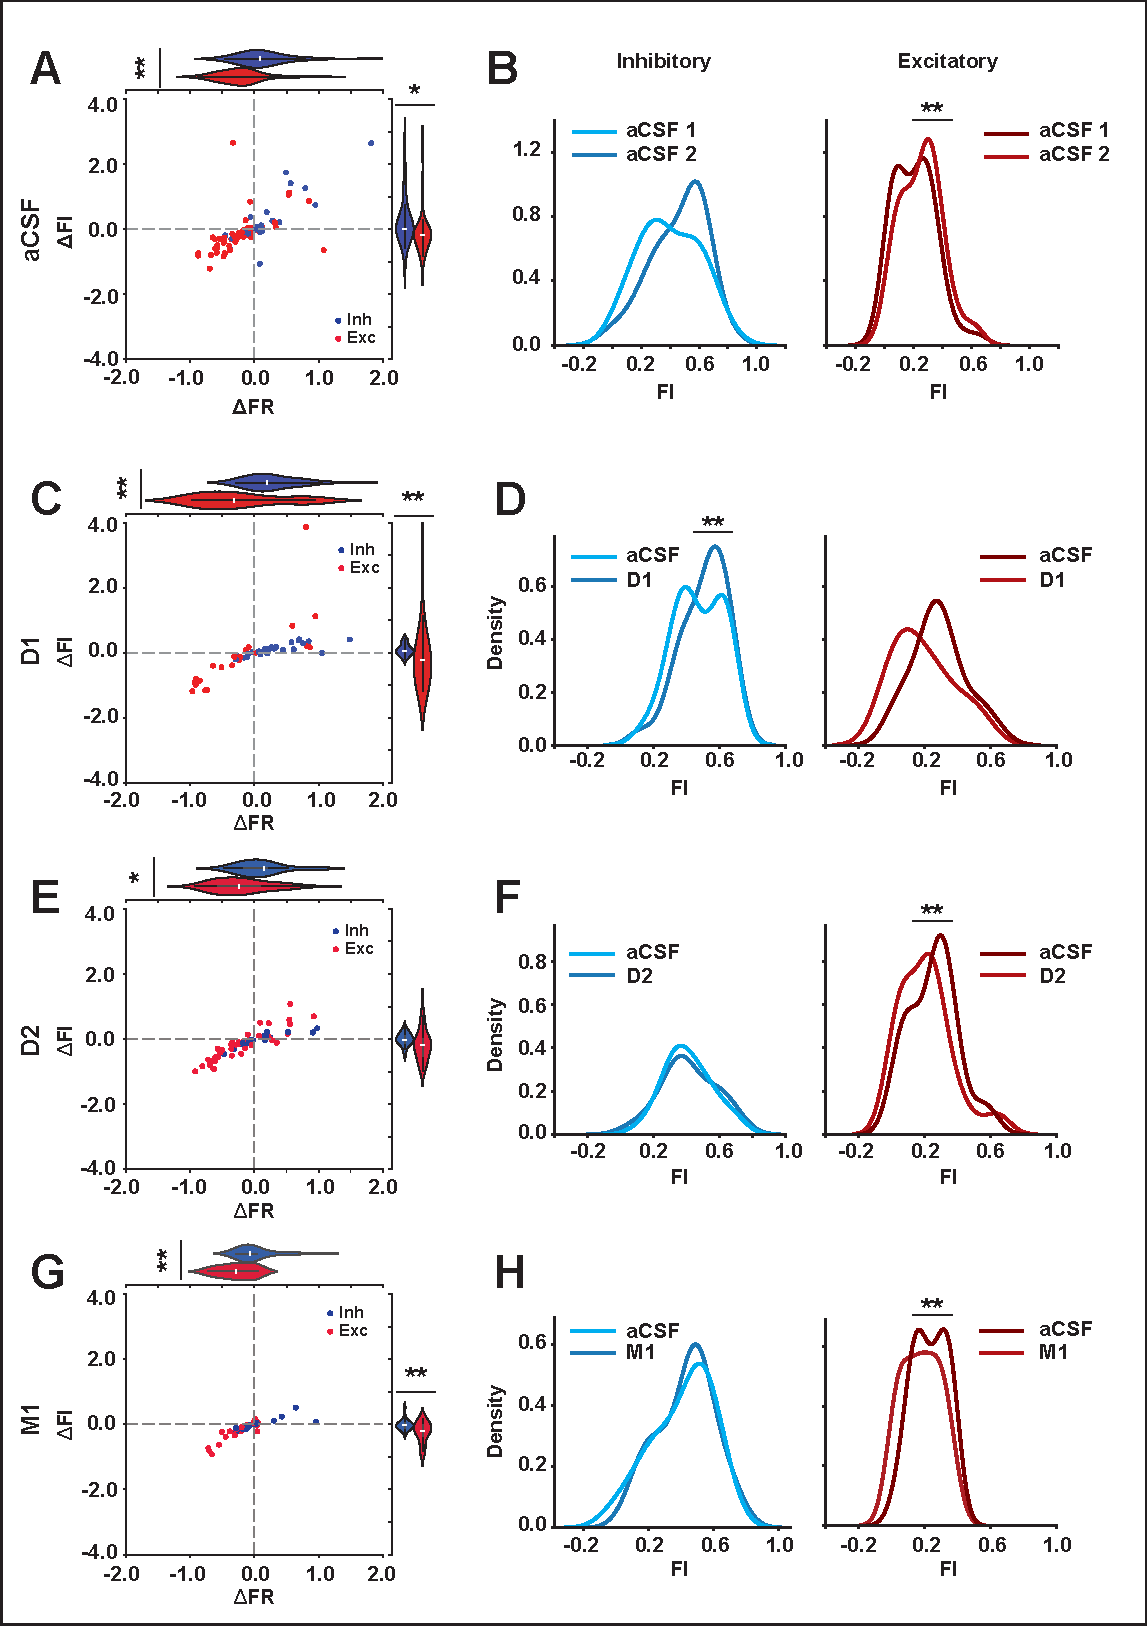
\includegraphics[width = 0.9\linewidth ]{Figures/Ch_3/Fig2.pdf}
	\caption{\textbf{Neuromodulation changes the amount of information transferred about the stimulus in a cell specific manner.}(\textbf{A}) 
    The scatter plot shows the relationship between change in firing rate and information transfer between two aCSF trials of the same neuron. 
    It can be seen that majority of Excitatory cells have decreases firing rate and decreased FI values as a result of consecutive recordings. 
    In contrast, inhibitory cells shows a much more diverse behavior. (\textbf{B}) KDE plot showing the distribution of measured FI for aCSF trial 1 
    and aCSF trial 2 conditions respectively. (\textbf{C}) Scatter plot (left) showing the normalized change in firing rate vs fractional information 
    as a result of D1 receptor activation. }
	\label{fig:Fig1_ref} % give each figure a logical label name
\end{figure}
\begin{figure}
(\textbf{D}) KDE plot showing the distribution of measured FI for aCSF and D1 conditions respectively. 
(\textbf{E}) Scatter plot (left) showing the normalized change in firing rate vs fractional information as a result of D2 receptor activation. 
(\textbf{F}) KDE plot showing the distribution of measured FI for aCSF and D2 conditions respectively. (\textbf{G}) Scatter plot (left) showing 
the normalized change in firing rate vs fractional information as a result of M1 receptor activation. (\textbf{H}) KDE plot showing the distribution 
of measured FI for aCSF and M1 conditions respectively. * $p<0.05$, ** $p<0.001$, *** $p<0.0001$.   
\end{figure}





\subsection{Specific receptor activation alters functional classification }

Neuromodulators are known to affect the intrinsic properties that may or may not depend on the input. For instance D2-R activation modulates excitability in motor cortex \cite{cousineau2020dopamine}. Neuronal functional classification which is classically studied using action potential and passive biophysical features, has been shown to change as a function of input to the neuron \cite{joshi2024understanding, hernath2019alternative, calcini2024electrical}. Also, we have shown in the previous section that neuromodulation (D1, D2, and M1 agonists) changes computation by changing amount of information transferred to a postsynaptic neuron in a cell-type specific manner. Therefore it is important to understand how functional attributes (passive, as well as input dependent) are altered by D1-R, D2-R and M1-R activation. Moreover, as functional attributes change, their assignment into different classes might also chance. Therefore, we look at how neural clustering based on functional attributes change as a result of neuromodulation. 

We first wanted to check if there is a drift present in the data as result of experimental setup while performing multiple trial (see Frozen Noise protocol section in Methods), for this we extracted the 4 functional attribute sets (AP, PB, AC and STA, see Table. \textbf{\ref{tab:functional_features}}) along with their waveforms from experiments with multiple aCSF trials and compared clustering the cells into subclasses (see Louvain+UMAP section in Methods) based on the acsf trial 1 and on acsf trial 2. The histogram in Fig. \ref{fig:S2} show that there is a high level of correspondence between clustering based on aCSF trial 1 and trial 2 for waveform and passive biophysical features. The low level of correspondence between the AP, AC, and STA results from inherent trial to trial variability present in the cell. We also show the manifold overlap between clustering based on trial 1 and trial 2 for all properties (see Fig. \textbf{\ref{fig:S2}}).   

After establishing the baseline for clustering similarity, we clustered D1-R, D2-R and M1-R agonist trials as well as their corresponding aCSF trials separately using UMAP+Louvain clustering (see Louvain+UMAP section in Methods as well as \cite{joshi2024understanding}) and measured the similarity between cluster labels for aCSF and agonist trials using adjusted mutual information score (AMI) see Louvain+UMAP section in Methods. We summarized the reliability of clusters between aCSF and agonist trials for excitatory neurons in case of D1-R activation in histogram (Fig. \textbf{\ref{fig:Fig2_ref} A.1}), it can be seen that AMI scores are consistently low for AP, PB, AC and STA, suggesting that functional attribute based clustering is altered as a result of D1-R activation, detailed co-classification matrices and average similarity within each cluster pair are provided in Fig. \textbf{\ref{fig:S1_ref} A}. 

We further explored how each attribute in the AP and PB attribute sets is altered as a result of D1-R activation, for passive biophysical properties (Fig. \textbf{\ref{fig:Fig2_ref} A.2}) we found that conductance (gL) (One Sided t-test: $p < 0.001$) and reset voltage (Vr) (One Sided t-test: $p < 0.05$) are significantly reduced as a result of D1-R activation. We then explored how adaptation current and linear input filter (STA) are altered as a result of D1-R modulation shown in Fig. \textbf{\ref{fig:Fig2_ref} A.3} and Fig. \textbf{\ref{fig:Fig2_ref} A.4}, the red curves represent D1 trials and black curves represent aCSF trials. To quantify the differences between D1 and aCSF trials, we calculated the rise time and peak values (see  Methods \ref{methods}) for both adaptation currents and STA. The joint plot Fig. \ref{fig:S5} shows the rise time and peak differences between D1 and aCSF trials for adaptation current and Fig. \ref{fig:S6} shows rise time and peak value for STA. The peak and rise time for adaptation current (AC paired t-test (decay time): $p = 0.4341$, AC paired t-test (peak): $p = 0.2444$) and STA (STA paired t-test (rise time): $p = 0.758$, STA paired t-test (peak): $p = 0.0514$) were found to not be significantly different between aCSF and D1 trials for excitatory neurons. This suggest that STA and adaptation currents are not altered significantly as a result of D1-R activation. 

We also performed a cosine similarity measurement within (between agonist-agonist or aCSF-aCSF) and across the aCSF and D1 trials for AC curves see Fig. \ref{fig:S7}, we performed a Kruskal--Wallis H test on three groups: within-aCSF, within-agonist, and across-aCSF and agonist conditions. The test revealed a significant effect of group based on similarity distributions ($H(2) = 15.3953$, $p = 4.53e-4$). Post hoc comparisons using Mann--Whitney U tests (Bonferroni-corrected for multiple comparisons) showed that:
\begin{itemize}
    \item The mean cosine similarity score was significantly higher for within aCSF compared to across-pair (aCSF-D1) comparisons ($U = 120654.00 $, $p = 3.17e-4$),
    \item Within D1 mean cosine similarity was also found to be significantly lower than across-pair (D1-aCSF) mean cosine similarity ($U = 153267.00$, $p = 0.0217$),
    \item We didn't observe a significant difference between the mean cosine similarity between within aCSF and D1 cosine similarity distributions ($U = 135299.00$, $p = 1.0$).
\end{itemize}

These findings indicate that neural representations are more consistent within conditions than across conditions, suggesting that D1 modulation significantly alters adaptation current consistently across the population.

Similar to adaptation current, we also performed a cosine similarity measurement within and across the aCSF and D1 trials for STA curves, we performed a Kruskal--Wallis H test on three groups: within-aCSF, within-agonist, and across-aCSF and agonist conditions. The test revealed a significant effect of group based on similarity distributions ($H(2) = 14.3199$, $p = 7.77e-4$).

Post hoc comparisons using Mann--Whitney U tests (Bonferroni-corrected for multiple comparisons) showed that:
\begin{itemize}
    \item Similarity scores were significantly higher within aCSF compared to across-pair comparisons ($U = 142428.00 $, $p = 7.44e-3$),
    \item D1 also showed significantly lower similarity than across-pair comparisons ($U = 134285.50$, $p = 1.95e-3$),
    \item We didn't observe a significant difference between aCSF and D1 mean cosine similarity distributions ($U = 142204.00$, $p = 1.0$).
\end{itemize}

These findings indicate that neural representations are more consistent within conditions than across conditions, suggesting that D1 modulation significantly alters the STA consistently across the population.

Finally, we assessed the effect of D1-R activation on action potential attributes (Fig. \textbf{\ref{fig:Fig2_ref} A.5}) which incorporates spiking dynamics, spiking threshold and AP height and width attributes for the excitatory population. We found that maximum ISI (one sided t-test: $t = 3.148$, $p = 4.49e-3$), mean ISI (one sided t-test: $t = 2.283$, $p = 0.0319$), instantaneous firing Rate (one sided t-test: $t = -3.826$, $p = 8.64e-4$) from the spiking dynamics are significantly altered as a result of D1-R activation. We performed similar analysis for D2 and M1 agonist trials and summarized the results in Fig. \ref{fig:S3_ref} and Fig. \ref{fig:S4_ref}. This was done to provide a template for understanding effect of the modulation on individual properties in a cell-type specific manner. Also, the D1-R are shown because they have the most number of samples.        

For inhibitory neurons, the effect on clustering in case of D1-R activation is shown in histogram (Fig. \textbf{\ref{fig:Fig2_ref} B.1}). It can be seen that AMI scores are consistently low for AP, PB, AC and STA, suggesting that functional attribute based clustering is altered as a result of D1-R activation, detailed co-classification matrices and average similarity within each cluster pair for each parameters is provided in Fig. \textbf{\ref{fig:S1_ref} A}. We further explored how each attribute set is altered as a result of D1-R activation. For passive biophysical properties (Fig. \textbf{\ref{fig:Fig2_ref} B.2}), we found that the conductance (gL) and the reset voltage (Vr) are significantly reduced (One sided t-test: p<0.001, p<0.05) as a result of D1-R activation. We then explored how adaptation current and linear input filter (STA) are altered as a result of D1-R modulation shown in Fig. \textbf{\ref{fig:Fig2_ref} B.3} and Fig. \textbf{\ref{fig:Fig2_ref} B.4}. As for the excitatory population, we calculated the rise time and peak values (see \ref{methods}) for both adaptation currents and STA. The joint plot Fig. \ref{fig:S5} shows the rise time and peak differences between D1 and aCSF trials for adaptation current and Fig. \ref{fig:S6} shows rise times and peak values for STA. The peak (paired t-test: $t = -1.195$, $p = 0.244$) and decay times (paired t-test: $t = 0.7966$, $p = 0.4341$) for adaptation currents were not found to be significantly different. For STA, the rise time was found to be significantly different between aCSF and D1 trials (paired t-test: $t = 2.454$, $p = 0.0208$) but the peak current was not significantly different for inhibitory neurons (paired t-test: $t = 1.834$, $p = 0.077$). This suggest that STAs and adaptation currents are not altered significantly as a result of D1-R activation. 

\clearpage
\begin{figure}[!htpb] % Do NOT use \begin{figure*}
	\centering
	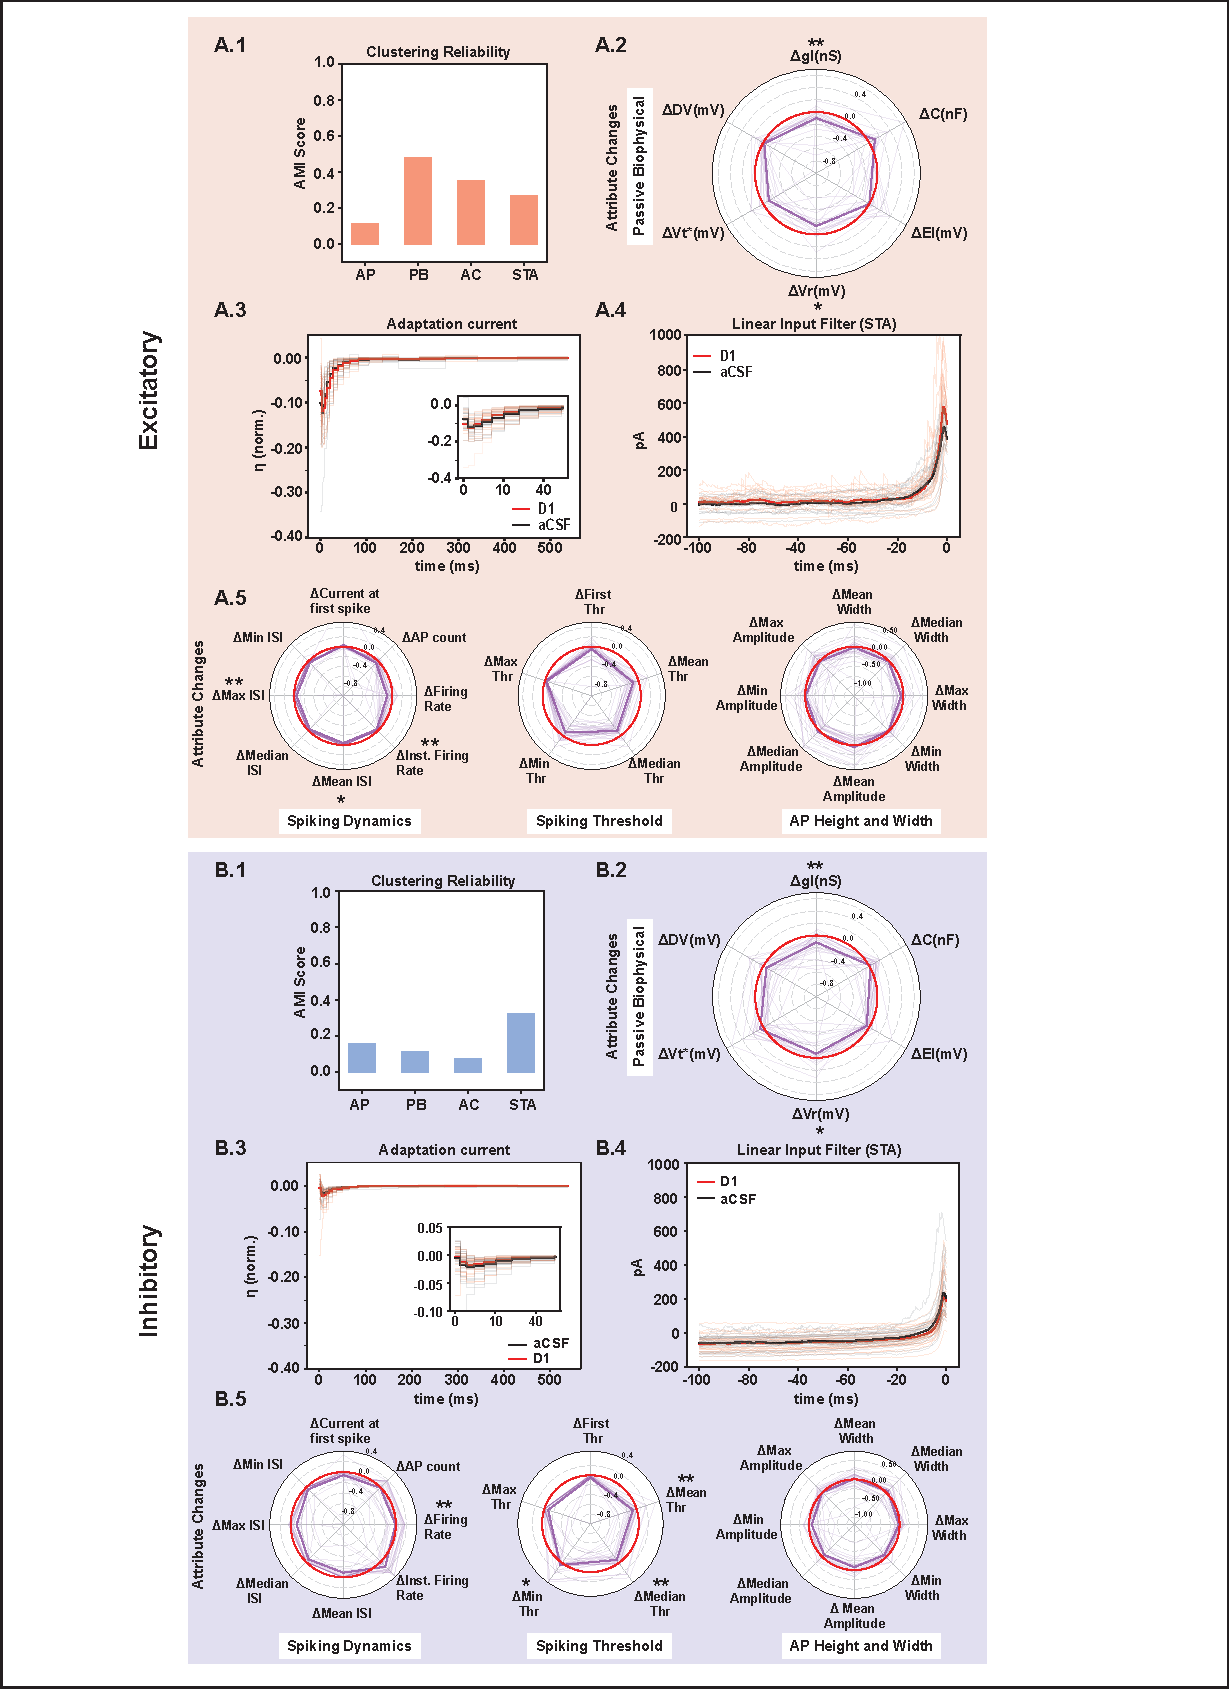
\includegraphics[width=0.9\textwidth]{Figures/Ch_3/Fig3.pdf} % for an image file 
    \caption{\textbf{D1-R activation changes functional clustering and attributes for both excitatory and inhibitory neurons.}(\textbf{A.1}) 
    Histogram shows the adjusted mutual information score between the clustering labels obtained for aCSF and D1 trials, the histogram shows 
a shift in cluster identities as a result of D1 receptor activation across four attributes. (\textbf{A.2}) shows the change in passive parameters with 
respect to control as a result of D1 receptor activation, normalized by the control trial values. (\textbf{A.3}) shows the adaptation current for control 
(black) and D1 (red), the mean is represented with darker curves. (\textbf{A.4}) shows the spike triggered average profile for aCSF (black) and D1 (red) 
trials, the mean is represented with a thick line. }
	\label{fig:Fig2_ref} % give each figure a logical label name
\end{figure}
    
\begin{figure}
(\textbf{A.5}) shows the change in action potential attribute sets with respect to control as a result 
of D1 receptor activation, normalized by the control trial values. With the mean marked represented with a thick line and the zero line is coloured in red. 
(\textbf{B.1-5}) Same as \textbf{A.1-5} but for inhibitory neurons. * $p<0.05$, ** $p<0.001$, *** $p<0.0001$.
\end{figure}


We also performed a cosine similarity measurement within and across the aCSF and D1 trials for AC curves and a Kruskal--Wallis H test on three groups to check for significant grouping: within-aCSF, within-agonist, and across-aCSF and agonist conditions. The test revealed a no significant effect between aCSF and D1 trials on similarity distributions ($H(2) = 2.0098$, $p = 0.3660$). These findings indicate that the AC is not altered as a result of D1 modulation. Similarly, we performed a cosine similarity measurement within and across the aCSF and D1 trials for STA curves. The test revealed a significant effect of group based on similarity distributions ($H(2) = 3.2486$, $p = 0.1970$). These findings indicate that the AC is not altered as a result of D1 modulation. Finally, we assessed the effect of D1-R activation on action potential attributes (Fig. \textbf{\ref{fig:Fig2_ref} B.5}) which incorporates spiking dynamics, spike threshold and AP height and width attributes for inhibitory population. We found that firing rate (one sided t-test: $t = 3.6275$, $p = 0.0011$) from the spiking dynamics subset is significantly altered, and also the mean threshold (one sided t-test: $t = 4.1205$, p = $3.03e-4$), median threshold (one sided t-test: $t = 4.361$, $p = 1.58e-4$) and minimum threshold (one sided t-test: $t = 2.443$, $p = 0.021$) from the spiking threshold set were significantly altered as result of D1-R activation.    

We wanted to further understand if there are sub groups of neurons that are altered differently in their action potential and passive biophysical attributes as a result of D1-R activation. For this, we clustered the change in AP and PB attributes between aCSF and D1 trials for both excitatory and inhibitory neurons and summarized our finding using polar plots with each set of attributes in Fig. \textbf{\ref{fig:Fig3_ref}}. Each curve represents a single neuron, colored with its respective cluster identity and the mean is represented with a thick line. It can be seen that there are 3 clusters of AP attributes for excitatory neurons and 4 clusters for inhibitory neurons. Similarly, we find 3 clusters each of PB attributes for both excitatory and inhibitory neurons. We also compared the overall similarity between clustering results based on aCSF trials and clustering the difference between aCSF and D1 trials for the 4 attribute sets using the AMI score between cluster labels. We summarized our findings in histogram shown in Fig. \ref{fig:Fig3_ref}. It can be seen that AMI score for both excitatory and inhibitory neurons are consistently low for all 4 attributes for both excitatory and inhibitory neurons. We performed a similar analysis for D2 and M1 agonist trials and summarized our findings in Fig. \textbf{\ref{fig:S8}} and Fig. \textbf{\ref{fig:S9}}.  




\clearpage
\begin{figure}[!htpb]
    \centering
    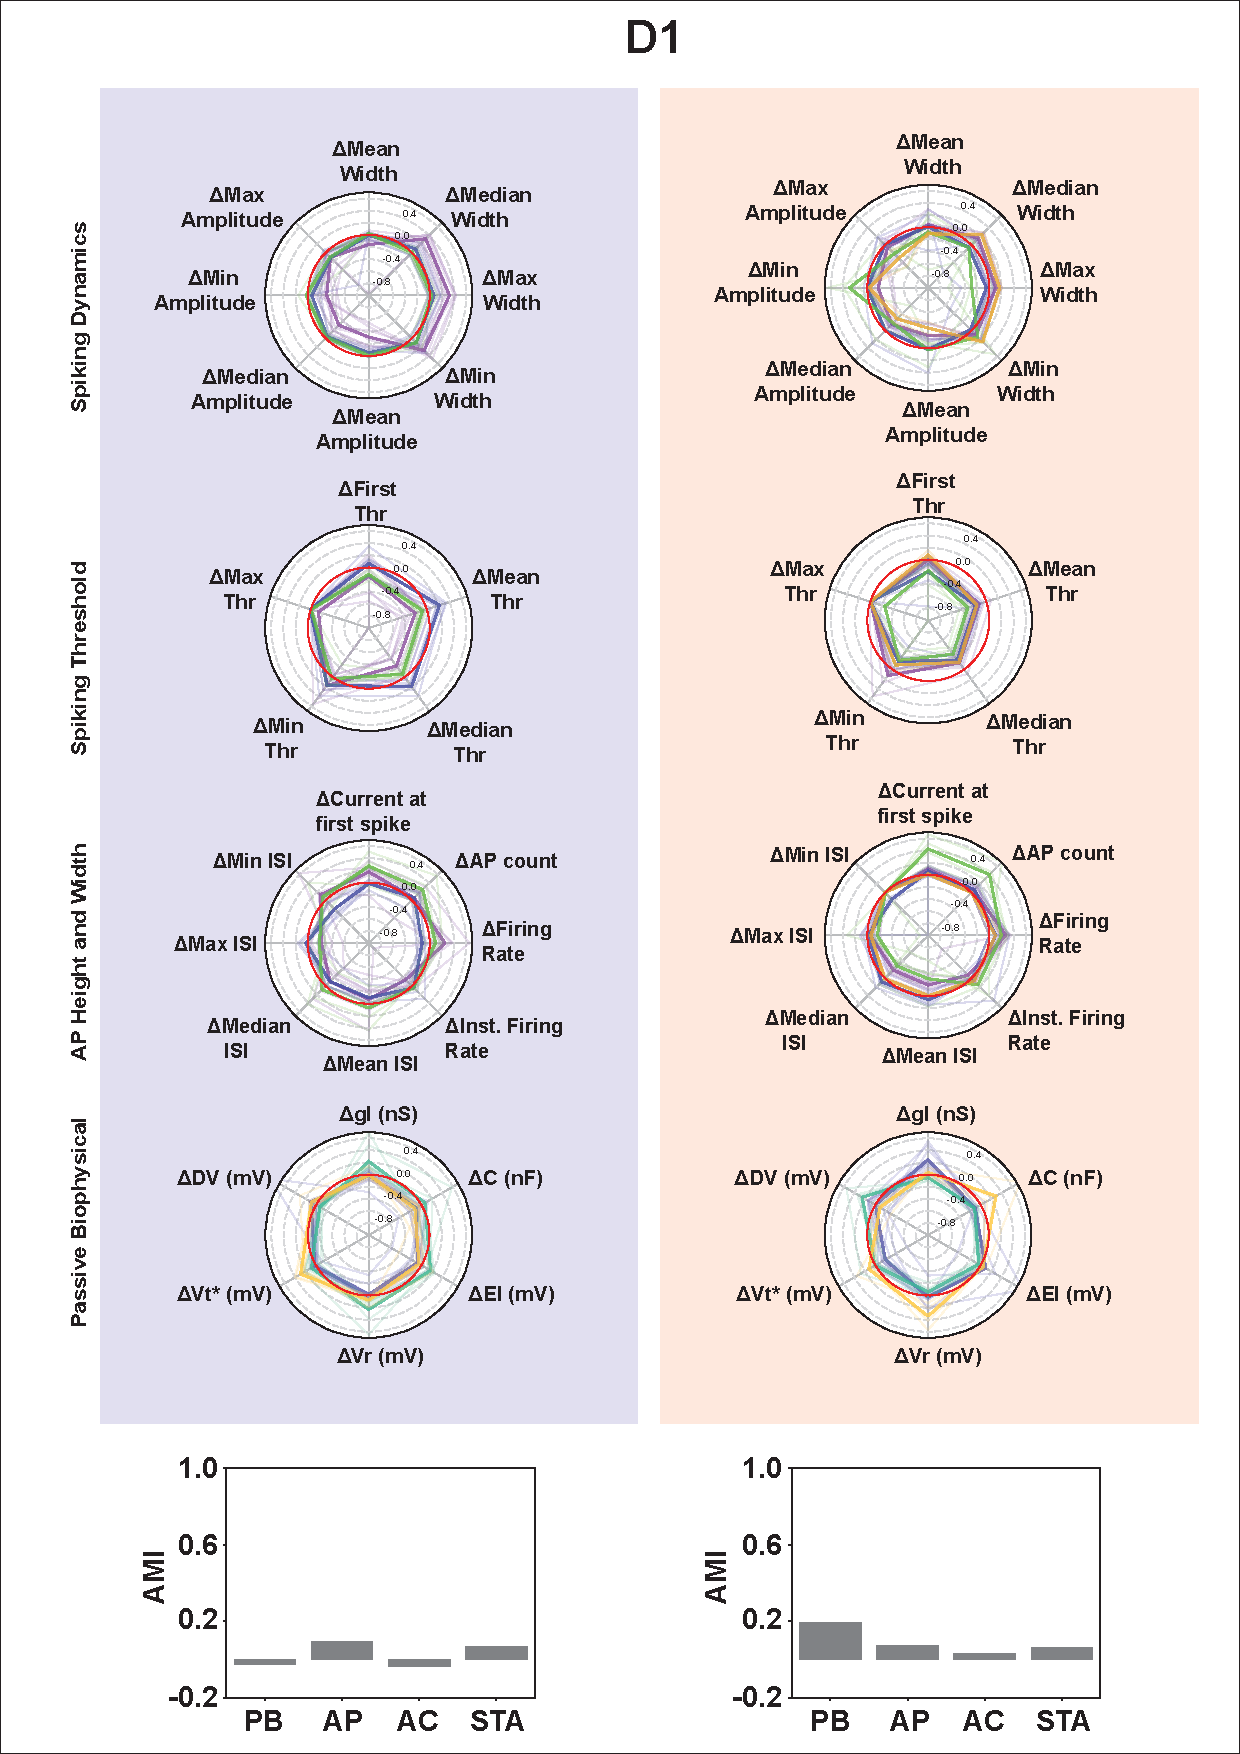
\includegraphics[width=0.9\linewidth]{Figures/Ch_3/Fig4.pdf}
    \caption{\textbf{Clustering based on differences between control and D1 trials for action potential and passive biophysical attributes reveals 
    subgroups of neurons getting modulated differently as a result of D1-R activation.}}
    \label{fig:Fig3_ref}
\end{figure} 

\begin{figure}
The polar plots show the clusters based on difference values between D1 and aCSF trials for action potential (subdivided into spiking dynamics, spiking threshold and AP height and width) and passive biophysical properties for both, excitatory (red background) and inhibitory (blue background). Each neuron is represented with a thin line and colored with their respective cluster label. The mean for each cluster is represented with a thick line. The histogram at the bottom shows the AMI score between cluster results using aCSF trials and the cluster results based on the difference between D1 and aCSF trials. 
\end{figure}

\subsection{Neuromodulation changes structured correlation between functional attributes in a cell-type as well as receptor type specific manner}



After showing that neuromodulation alters stimulus encoding in a cell-type specific manner and reorganizes functional subpopulations in cortical circuits, we further asked how neuromodulation (dys)regulates specific sets of neuronal properties (AP, PB, AC, and STA) which together span the high-dimensional correlated structure of functional properties neurons. While clustering revealed how neuromodulation reshapes functional subtypes, it did not address whether these changes reflect coordinated shifts in the underlying feature sets. Understanding how these attributes shift in response to receptor-specific activation provides a more mechanistic insight into how computational capacities are reconfigured. Specifically, we asked: are these properties modulated in isolation, or are they co-regulated in a coordinated fashion that might explain observed changes in encoding? To establish this, we applied multi-set correlation and factor analysis (MCFA) to our dataset, first on aCSF (control) trials and each agonist trial set respectively. We summarized the results of shared, private and residual variance using a stacked histogram (Fig. \textbf{\ref{fig:Fig4_ref}}). In this analysis, when individual feature sets exhibit a high shared variance, this means that the features are functionally coordinated: changes in one set tend to co-vary with changes in others. In contrast, when feature sets exhibit a high private variance, it suggests that the features are relatively independent i.e, uncoordinated, meaning changes in one set do not systematically correspond to changes in the others, or a feature with a high private variance varies independently from the other features. A high residual signifies either noise or a complex non-linear relationship not captured by a linear method such as MCFA (Summarized in Table.\ref{tab:mcfa_inerpretation}). 
\begin{table}[h]
    \centering
    \begin{tabular}{p{4cm}|p{8cm}}
    \hline
    Variance type & Description \\ 
    \hline
     Shared variance &  Variance correlated across all feature sets (indicating coordinated modulation)\\
     Private variance & Variance unique to each set (indicating functional independence) \\
     Residual variance & Unexplained variance (potential noise or non-linear effects) \\
    \hline
    \end{tabular}
    \caption{A brief summary of MCFA interpretation and meaning of different variances and residuals.}
    \label{tab:mcfa_inerpretation}
\end{table}
To account for the sample size imbalance, we performed a bootstrapped random sub-sampling of aCSF trials equal to the agonist set with minimum number of trials, and repeated MCFA a 100 times using random subsets. The reported aCSF values reflect the mean shared/private/residual variance across bootstraps. Standard deviations (or confidence intervals) are included in Tables. \ref{tab:specific_values_exc} \& \ref{tab:specific_values_inh} to reflect the variability in control estimates. We present our findings using a stacked histogram for each condition in a cell type specific manner. 

\subsubsection{D1-R agonist}
First we looked at the effect of D1-agonist. It can be seen in Fig. \ref{fig:Fig4_ref} that the private variance for excitatory population decreases for AP, PB and AC sets except for STA, for which it sharply increases (aCSF: $16.7742\%$ $\rightarrow$ D1: $73.9663\%$) compared to aCSF trials (see Table.\ref{tab:specific_values_exc} and Figure \ref{fig:Fig4_ref} \textbf{A-B}) upon D1 receptor activation. The shared variance reduces sharply compared to aCSF for AC (aCSF: $15.8369\%$ $\rightarrow$ D1: $6.9056\%$) and STA (aCSF: $23.6072\%$ $\rightarrow$ D1: $9.5260 \%$) sets for the excitatory population. This suggests that D1-R activation makes the STA more independent compared to the other attributes. The shared variance for AP an PB has slightly increased, suggesting that PB and AP attributes become more coordinated. 
We observe a dramatically different effect in the inhibitory population compared to the excitatory counterpart. The shared variance increases sharply for the STA set (aCSF: $23.6595 \%$ $\rightarrow$ D1: $46.2345\%$) and also for the AC set (aCSF: $26.9763\%$ $\rightarrow$ D1: $44.4749\%$) (see Figure. \ref{fig:Fig4_ref}\textbf{A-B} and Table. \ref{tab:specific_values_inh}), while the private variance decreases for these attributes, suggesting that the AC and STA become functionally coordinated with the latent space, therefore with AP and PB properties. It is also worth noticing that the private variance decreases sharply for the AP (aCSF: $14.9272\%$ $\rightarrow$ D1: $0.8297\%$) and PB (aCSF: $13.1228\%$ $\rightarrow$ D1: $3.9880\%$). Similarly, the shared variances decrease for both the AP and PB (see Figure. \ref{fig:Fig4_ref}\textbf{A-B} and Table. \ref{tab:specific_values_inh}) suggesting the interaction between these two sets show a weakened linear correlation with other feature sets. 

In summary, the effect of D1-R is cell-type specific and nuanced, increasing the coordination between STA and AC properties in inhibitory neurons, while decreasing coordination for excitatory STA with the rest of the attribute sets.

\subsubsection{D2-R agonist}

In order to study the effect of D2-R activation, we analyzed D2-R trials using MCFA in a similar manner to the D1-R activation and present the results in comparison with aCSF trials (see Fig. \ref{fig:Fig4_ref}\textbf{A-C} and Table. \ref{tab:specific_values_exc}). 

We observe that D2-R modulates the coordination between functional attributes in a more subtle manner than D1-R for excitatory neurons: the private variance for STA increases with D2-R activation (aCSF: $57.7380\%$ $\rightarrow$ D2: $71.2200\%$), and at the same time the shared variance between AC and AP attributes increases (see Fig. \ref{fig:Fig4_ref}\textbf{A-C} and Table. \ref{tab:specific_values_exc}). Private variance on the other hand decreases drastically for AP, AC and PB attributes as also observed in case of D1. The stark increase in private variance in case of STA needs to be highlighted. This suggests that D2-R activation makes AP and AC properties more coordinated, while making STA and PB more functionally decoupled from other attributes. 

In the case of the inhibitory neurons, the modulation is rather straight-forward. The private variance for all attributes except for the AC decreases and the shared variance increases for all the attributes except for AP attributes. This suggests that D2-R overall makes the functional properties more coupled for inhibitory population.     

In summary, the effect of D2-R activation is cell-type specific as in the case of D1-R case. Increasing the coordination between AP and AC properties in the excitatory population while making the STA independent and making the PB, STA and AC sets coordinated for the inhibitory population.


\subsubsection{Muscarinic M1-R agonist}

In the case of M1 receptor activation, we observe that the shared variance increases for AP (aCSF: $30.8543\%$ $\rightarrow$ M1: $66.0431\%$) an AC (aCSF: $15.8369\%$ $\rightarrow$ M1: $35.0802\%$) properties similar to D2 for excitatory neurons and decreases for PB and STA (see Fig. \ref{fig:Fig4_ref}\textbf{A-D} and Table. \ref{tab:specific_values_exc}). This suggests that AC and AP attributes become coordinated and PB and STA properties become more independent as a result of M1-R activation. On the other hand, the private variance decreases for all the attributes except for PB. Another important thing to notice is that the residual for STA increases sharply, we suspect that this is due to a decrease in firing rate as a result of M1-R activation, that increases the noise in STA measurement. 

For inhibitory neurons, the shared variance increases for all sets except for AC, suggesting a stronger functional coordination (see Fig. \ref{fig:Fig4_ref}\textbf{A-D} and Table. \ref{tab:specific_values_inh}). Surprisingly, the private variance increases sharply for the AC, suggesting a decoupling with the rest of the attributes set.    

In summary, the effect of Muscarinic M1-R activation is cell-type specific as well but different from D1-R and D2-R, increasing coordination between AP and AC properties and making PB set independent in excitatory population and making STA independent while making AP, STA and PB sets coordinated (increasing independence for AC) and for inhibitory population.

\subsubsection{Summary}
\begin{table}
    \centering
    \begin{tabular}{p{2cm}|p{2cm}|p{8cm}}
    \hline
        Receptor & Cell-type & Effect \\
    \hline
        D1-R     & Excitatory & Increases coordination between AP and PB and makes STA independent. \\
                 & Inhibitory & Increases coordination between AC and STA and reduces linearity.\\
                 & &  between AP and PB sets. \\
        
        D2-R     & Excitatory & Increases coordination between AP and AC and makes STA independent. \\
                 & Inhibitory & Makes PB, AC and STA coordination stronger. \\
        
        M1-R     & Excitatory & Makes AP and AC coordination stronger while making PB more  \\
        & & independent. \\
                 & Inhibitory & Makes coordination between AP, PB and STA stronger while making \\ 
                 & &  AC independent.         \\
    \hline            
    \end{tabular}
    \caption{A summary of findings from MCFA for each receptor type. }
    \label{tab:MCFA_summary}
\end{table}

In summary, our MCFA analysis reveals that neuromodulation alters the coordination structure between key functional attributes -- action potential dynamics, passive biophysics, adaptation currents, and input filtering in a receptor and cell-type-specific manner. In excitatory neurons, D1-R and D2-R activation selectively increase the independence of input feature selectivity (STA), while promoting a greater coupling between output-related features such as action potentials and adaptation currents. In contrast, inhibitory neurons exhibited a consistent increase in coordination across all functional domains under D1-R, D2-R, and M1-R activation, with a marked reduction in private variance, suggesting a shift towards more integrated and cohesive functional states. Notably, M1-R activation produced a unique pattern: excitatory neurons exhibited strengthened AP–AC coupling alongside increased independence in passive and input features, while inhibitory neurons showed a widespread coordination (except for adaptation currents, which became more decoupled). Overall, the ratio of shared to private variance increased across all receptor conditions relative to control, indicating that neuromodulators generally enhance the global coordination of neuronal features. These findings highlight the diverse strategies by which neuromodulators reshape the functional architecture of neurons—either by reinforcing coordinated, stable encoding in inhibitory populations or by promoting selective flexibility and specialization in excitatory neurons.
A complete summary is shown in Table. \ref{tab:MCFA_summary}.



\clearpage
\begin{figure}[!htpb] % Do NOT use \begin{figure*}
	\centering
	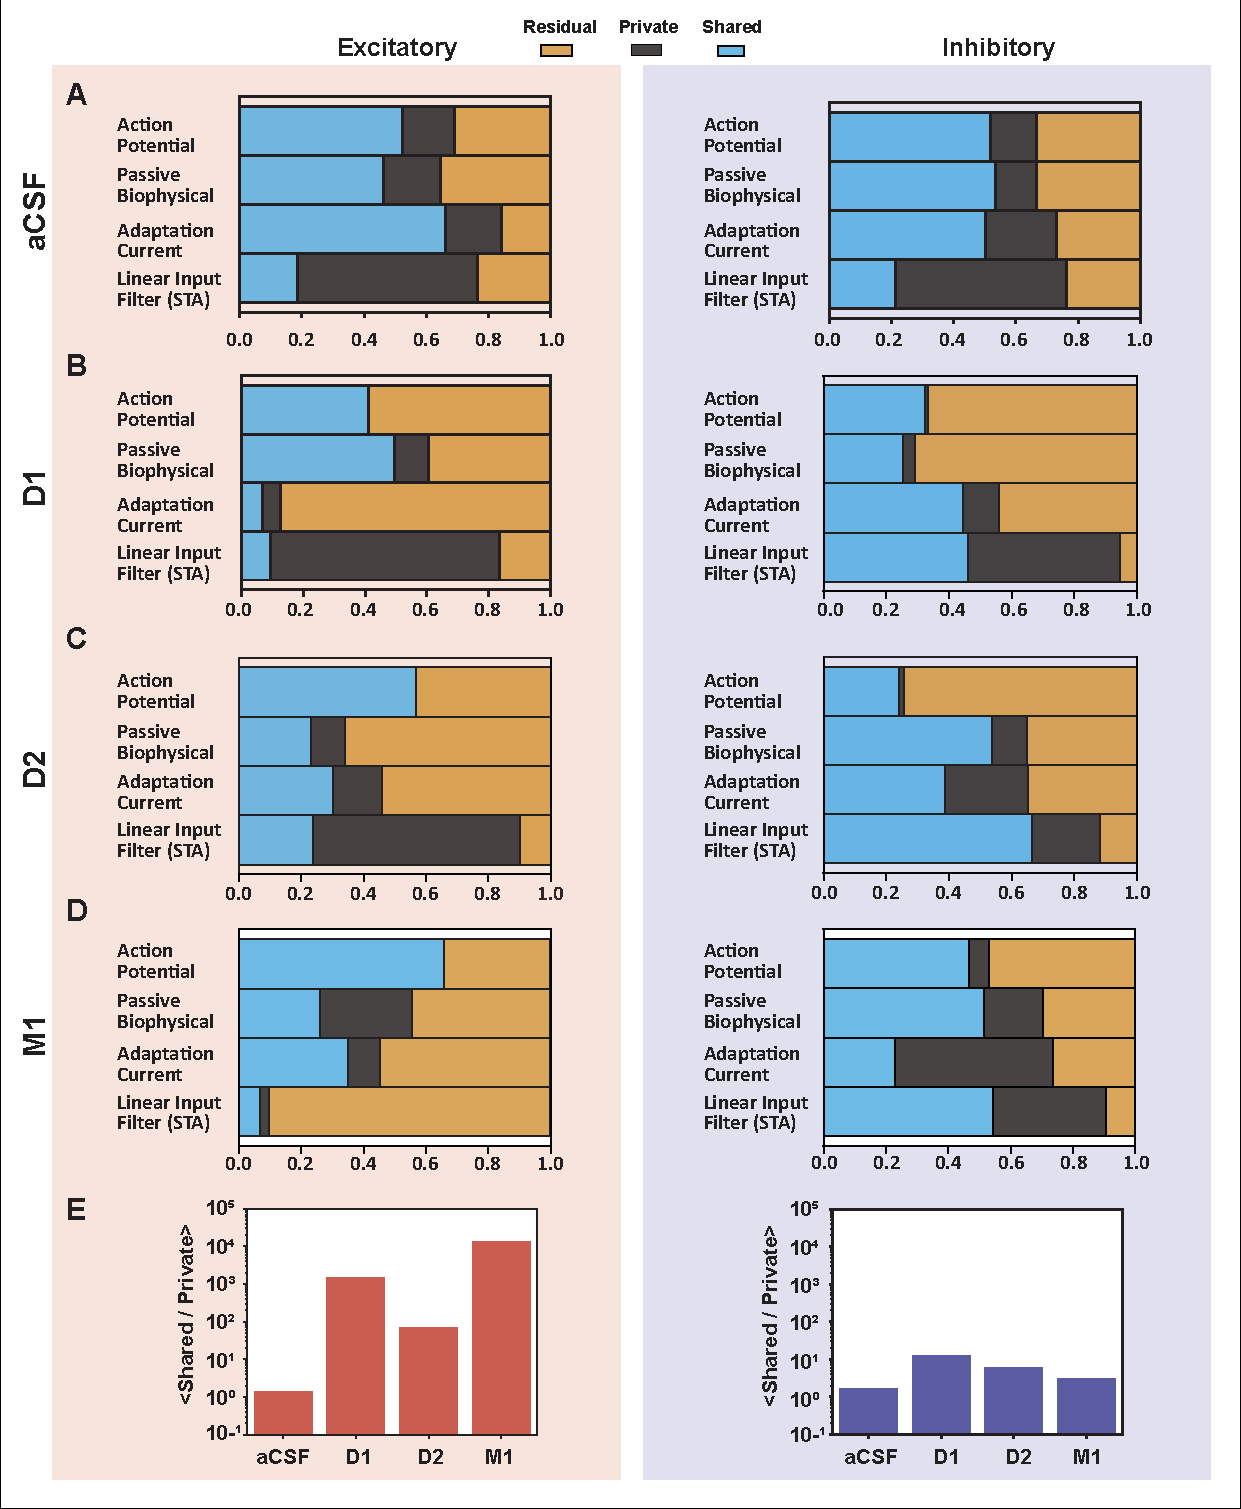
\includegraphics[width=\linewidth]{Figures/Ch_3/Fig5.pdf}
    \caption{\textbf{Correlation between functional attributes changes as a result of D1, D2 and M1 receptor activation compared 
    to control in both excitatory and inhibitory neurons.} {\textbf{A} Left stacked bar-plot shows the MCFA results for aCSF-excitatory trials and on the right is the aCSF-inhibitory trials. 
 \textbf{B} Left stacked bar-plot shows the MCFA results of D1-excitatory trials and the corresponding inhibitory trials is on the right. 
 \textbf{C-D} show the excitatory and inhibitory MCFA results for D2 and M1 agonist trials respectively. Excitatory trials are on the 
 left and inhibitory on the right. \textbf{E} Left histogram shows the ratio of shared and private variance for control and each agonist 
 conditions in the excitatory population. Similarly right histogram shows the ratio of shared over private variance for inhibitory 
 population for each agonist condition.}}
	\label{fig:Fig4_ref} % give each figure a logical label name
\end{figure}
% \begin{figure}
%  {\textbf{A} Left stacked bar-plot shows the MCFA results for aCSF-excitatory trials and on the right is the aCSF-inhibitory trials. 
%  \textbf{B} Left stacked bar-plot shows the MCFA results of D1-excitatory trials and the corresponding inhibitory trials is on the right. 
%  \textbf{C-D} show the excitatory and inhibitory MCFA results for D2 and M1 agonist trials respectively. Excitatory trials are on the 
%  left and inhibitory on the right. \textbf{E} Left histogram shows the ratio of shared and private variance for control and each agonist 
%  conditions in the excitatory population. Similarly right histogram shows the ratio of shared over private variance for inhibitory 
%  population for each agonist condition.}
% \end{figure}



%%%%%%%%%%%%%%%%%%%%%%%%%%%%%%%%%%%%%%%%%%%%%%%%%%%%%%%%%%%%%%%%%%%%%%%%
%%%%%%%%%%%%%%%%%%%%%%%%%%%%%% Discussion %%%%%%%%%%%%%%%%%%%%%%%%%%%%%%
%%%%%%%%%%%%%%%%%%%%%%%%%%%%%%%%%%%%%%%%%%%%%%%%%%%%%%%%%%%%%%%%%%%%%%%%

\section{Discussion}


In this study, we aimed to investigate how neuromodulation, specifically through dopamine (D1R, D2R) and acetylcholine (M1R) receptor activation, alters the functional properties of cortical neurons beyond traditional measures of excitability. Using frozen noise stimulation based single-cell in-vitro somatic recordings from layer 2/3 of the mouse somatosensory cortex, we extracted four functional feature sets comprising action potential (AP), passive biophysical (PB), adaptation currents (AC), and linear input filter via a spike-triggered average (STA). This approach enabled us to study the impact of neuromodulation across multiple physiological domains within and across neuronal subtypes.

\subsubsection{Receptor-Specific Neuromodulation Reshapes Functional Architecture in Distinct Cell Types}

Our analyses revealed that dopaminergic and cholinergic receptor activation altered the correlation structure among functional attributes, and these effects were excitatory/inhibitory cell-type specific. For inhibitory neuron\textbf{s}, D1R and D2R activation increased inter-attribute correlations, suggesting a convergence of functional attributes under neuromodulatory influence. In contrast, excitatory neurons displayed decreased correlations under D1R activation, indicating a decoupling of intrinsic and encoding features. This suggests that dopaminergic modulation sharpens functional coherence in inhibitory neurons while increasing functional independence in excitatory neurons. 

These results extend previous findings that D1R activation increases firing in both excitatory and inhibitory neurons in prefrontal and motor cortices~\cite{seamans2004principal, tritsch2012dopaminergic,anastasiades2019cell}, by showing that in the sensory cortex, such modulation also reorganizes functional coupling between key electrophysiological domains. Inhibitory neurons, under D1R and D2R activation, exhibited stronger coupling between passive properties, AP dynamics, and linear input filtering; suggesting that neuromodulation may reduce heterogeneity and impose a more unified computational role. This aligns with the hypothesis that dopamine can increase synchronization and gain control within inhibitory networks, potentially sharpening their influence on local circuits \cite{gao2003selective,morozova2016dopamine,seamans2001dopamine}.

Interestingly, we observed similar coupling effects under M1R activation, pointing to a convergent mechanism across dopaminergic and cholinergic systems in shaping the internal structure of inhibitory neuron function. The decoupling observed in excitatory neurons, particularly under D1R, may reflect a shift toward greater computational flexibility or specialization, allowing for more diverse input-output transformations. These effects may be a substrate for dynamic control of cortical processing modes, such as switching between attentive and exploratory states.

\subsubsection{Functional Clustering and Heterogeneous Modulation of Neuronal Identity}

To examine how these neuromodulatory changes reorganize functional neuron types, we applied UMAP-Louvain clustering to the high-dimensional feature sets before and after receptor activation. Our results show that agonist application drastically alters functional clustering, suggesting that receptor-specific modulation reshapes neuronal identities in both excitatory and inhibitory populations.

Importantly, the modulatory effects were not uniform, but heterogeneous within cell types, implying that neuromodulation acts in a subtype-specific manner. This is consistent with recent work showing volume transmission and receptor expression gradients as mechanisms for differential modulation across cell types~\cite{ozccete2024mechanisms}. By clustering neurons based on their change vectors (difference between agonist and control), we identified distinct subpopulations exhibiting coordinated shifts in AP and passive properties, reinforcing the idea that neuromodulation reconfigures the functional state space of neurons rather than simply scaling their excitability.

We also found that adaptation currents and STAs became more homogeneous in excitatory neurons compared to inhibitory neurons following neuromodulation. This suggests that although both populations undergo modulation, excitatory neurons may be pushed toward a more constrained encoding regime, possibly to provide stability in coding  under varying network conditions. Nonetheless, the core distinction between excitatory and inhibitory populations remained intact, highlighting the robustness of intrinsic identity despite substantial functional plasticity. We speculate that a modeling effort superimposing neuromodulatory affects on a balanced networks would reveal the implication of neuromodulatory alteration on the balance excitation-inhibition and therefore the shift that neuromodulation can cause.    

\subsubsection{Neuromodulation Selectively Alters Information Transfer}

While neuromodulators are known to affect neuronal excitability, less is known about how such changes impact information transmission. Using the frozen noise protocol~\cite{zeldenrust2017estimating}, we estimated fractional information (FI) between stimulus and spike train for each neuron under different receptor conditions.

Our key finding is that neuromodulation alters information transfer in a cell-type and receptor-specific manner. Specifically, D1R and M1R activation significantly decreased FI in excitatory neurons, while D2R activation increased FI in inhibitory neurons. This suggests that excitatory and inhibitory neurons are differentially engaged by neuromodulators to redistribute information processing roles. Moreover, FI variance increased in excitatory neurons under D1R, implying a diversification of encoding strategies, whereas inhibitory neurons exhibited more stable and coordinated changes.

These findings underscore an important result that modulation of biophysical and spike-generating properties has direct consequences on the information transfer and encoding of neurons. Neuromodulators do not simply shift the gain of neurons, they reconfigure how inputs are integrated and transformed into outputs, thus shaping the flow of information through cortical networks. This raises exciting new questions about how neuromodulatory systems shape perceptual inference, attention, and learning by dynamically allocating information processing across cell types.

\subsubsection{Limitations and Future Directions}

Our study, while comprehensive, has several important limitations. First, our recordings were limited to the soma, whereas neuromodulation often targets synaptic and dendritic compartments, which could substantially influence neuronal input-output transformations. Second, our analysis is constrained by sample size and cortical region, necessitating broader recordings across layers and brain areas to validate the generality of our findings.

Most critically, neuromodulatory systems are highly degenerate: the same ion channel can be targeted by multiple modulators, and a single neuromodulator can affect many channels and cellular processes. Thus, our receptor-specific results represent only a partial view of the underlying modulatory landscape. Future work should incorporate multi-receptor interactions, consider temporal dynamics of modulation, and examine how these single-cell changes propagate to network-level phenomena such as synchrony, attractor stability, and behavioral output.

\subsubsection{Conclusion}

Together, our findings reveal that D1, D2, and M1 receptor activation differentially reorganizes the biophysical, adaptive, and encoding properties of excitatory and inhibitory neurons in layer 2/3 of the somatosensory cortex. Neuromodulation can couple or decouple domains of neuronal function, alter functional classification, and modulate information transmission in a subtype-specific manner. These effects likely support context-dependent reconfiguration of cortical computation and offer a new window into how global modulatory signals dynamically orchestrate diverse local circuit functions.



\newpage
\begin{spacing}{1.0} % Set the line spacing to single spacing
\fontsize{8pt}{8pt}\selectfont
\bibliographystyle{apalike} %%%%Changed
\renewcommand{\bibname}{References}
\bibliography{All_bibtex} %%%%Changed
\end{spacing}